% Options for packages loaded elsewhere
% Options for packages loaded elsewhere
\PassOptionsToPackage{unicode}{hyperref}
\PassOptionsToPackage{hyphens}{url}
\PassOptionsToPackage{dvipsnames,svgnames,x11names}{xcolor}
%
\documentclass[
  letterpaper,
  DIV=11,
  numbers=noendperiod]{scrartcl}
\usepackage{xcolor}
\usepackage{amsmath,amssymb}
\setcounter{secnumdepth}{-\maxdimen} % remove section numbering
\usepackage{iftex}
\ifPDFTeX
  \usepackage[T1]{fontenc}
  \usepackage[utf8]{inputenc}
  \usepackage{textcomp} % provide euro and other symbols
\else % if luatex or xetex
  \usepackage{unicode-math} % this also loads fontspec
  \defaultfontfeatures{Scale=MatchLowercase}
  \defaultfontfeatures[\rmfamily]{Ligatures=TeX,Scale=1}
\fi
\usepackage{lmodern}
\ifPDFTeX\else
  % xetex/luatex font selection
\fi
% Use upquote if available, for straight quotes in verbatim environments
\IfFileExists{upquote.sty}{\usepackage{upquote}}{}
\IfFileExists{microtype.sty}{% use microtype if available
  \usepackage[]{microtype}
  \UseMicrotypeSet[protrusion]{basicmath} % disable protrusion for tt fonts
}{}
\makeatletter
\@ifundefined{KOMAClassName}{% if non-KOMA class
  \IfFileExists{parskip.sty}{%
    \usepackage{parskip}
  }{% else
    \setlength{\parindent}{0pt}
    \setlength{\parskip}{6pt plus 2pt minus 1pt}}
}{% if KOMA class
  \KOMAoptions{parskip=half}}
\makeatother
% Make \paragraph and \subparagraph free-standing
\makeatletter
\ifx\paragraph\undefined\else
  \let\oldparagraph\paragraph
  \renewcommand{\paragraph}{
    \@ifstar
      \xxxParagraphStar
      \xxxParagraphNoStar
  }
  \newcommand{\xxxParagraphStar}[1]{\oldparagraph*{#1}\mbox{}}
  \newcommand{\xxxParagraphNoStar}[1]{\oldparagraph{#1}\mbox{}}
\fi
\ifx\subparagraph\undefined\else
  \let\oldsubparagraph\subparagraph
  \renewcommand{\subparagraph}{
    \@ifstar
      \xxxSubParagraphStar
      \xxxSubParagraphNoStar
  }
  \newcommand{\xxxSubParagraphStar}[1]{\oldsubparagraph*{#1}\mbox{}}
  \newcommand{\xxxSubParagraphNoStar}[1]{\oldsubparagraph{#1}\mbox{}}
\fi
\makeatother


\usepackage{longtable,booktabs,array}
\newcounter{none} % for unnumbered tables
\usepackage{calc} % for calculating minipage widths
% Correct order of tables after \paragraph or \subparagraph
\usepackage{etoolbox}
\makeatletter
\patchcmd\longtable{\par}{\if@noskipsec\mbox{}\fi\par}{}{}
\makeatother
% Allow footnotes in longtable head/foot
\IfFileExists{footnotehyper.sty}{\usepackage{footnotehyper}}{\usepackage{footnote}}
\makesavenoteenv{longtable}
\usepackage{graphicx}
\makeatletter
\newsavebox\pandoc@box
\newcommand*\pandocbounded[1]{% scales image to fit in text height/width
  \sbox\pandoc@box{#1}%
  \Gscale@div\@tempa{\textheight}{\dimexpr\ht\pandoc@box+\dp\pandoc@box\relax}%
  \Gscale@div\@tempb{\linewidth}{\wd\pandoc@box}%
  \ifdim\@tempb\p@<\@tempa\p@\let\@tempa\@tempb\fi% select the smaller of both
  \ifdim\@tempa\p@<\p@\scalebox{\@tempa}{\usebox\pandoc@box}%
  \else\usebox{\pandoc@box}%
  \fi%
}
% Set default figure placement to htbp
\def\fps@figure{htbp}
\makeatother


% definitions for citeproc citations
\NewDocumentCommand\citeproctext{}{}
\NewDocumentCommand\citeproc{mm}{%
  \begingroup\def\citeproctext{#2}\cite{#1}\endgroup}
\makeatletter
 % allow citations to break across lines
 \let\@cite@ofmt\@firstofone
 % avoid brackets around text for \cite:
 \def\@biblabel#1{}
 \def\@cite#1#2{{#1\if@tempswa , #2\fi}}
\makeatother
\newlength{\cslhangindent}
\setlength{\cslhangindent}{1.5em}
\newlength{\csllabelwidth}
\setlength{\csllabelwidth}{3em}
\newenvironment{CSLReferences}[2] % #1 hanging-indent, #2 entry-spacing
 {\begin{list}{}{%
  \setlength{\itemindent}{0pt}
  \setlength{\leftmargin}{0pt}
  \setlength{\parsep}{0pt}
  % turn on hanging indent if param 1 is 1
  \ifodd #1
   \setlength{\leftmargin}{\cslhangindent}
   \setlength{\itemindent}{-1\cslhangindent}
  \fi
  % set entry spacing
  \setlength{\itemsep}{#2\baselineskip}}}
 {\end{list}}
\usepackage{calc}
\newcommand{\CSLBlock}[1]{\hfill\break\parbox[t]{\linewidth}{\strut\ignorespaces#1\strut}}
\newcommand{\CSLLeftMargin}[1]{\parbox[t]{\csllabelwidth}{\strut#1\strut}}
\newcommand{\CSLRightInline}[1]{\parbox[t]{\linewidth - \csllabelwidth}{\strut#1\strut}}
\newcommand{\CSLIndent}[1]{\hspace{\cslhangindent}#1}



\setlength{\emergencystretch}{3em} % prevent overfull lines

\providecommand{\tightlist}{%
  \setlength{\itemsep}{0pt}\setlength{\parskip}{0pt}}



 


\KOMAoption{captions}{tableheading}
\makeatletter
\@ifpackageloaded{caption}{}{\usepackage{caption}}
\AtBeginDocument{%
\ifdefined\contentsname
  \renewcommand*\contentsname{Table of contents}
\else
  \newcommand\contentsname{Table of contents}
\fi
\ifdefined\listfigurename
  \renewcommand*\listfigurename{List of Figures}
\else
  \newcommand\listfigurename{List of Figures}
\fi
\ifdefined\listtablename
  \renewcommand*\listtablename{List of Tables}
\else
  \newcommand\listtablename{List of Tables}
\fi
\ifdefined\figurename
  \renewcommand*\figurename{Fig}
\else
  \newcommand\figurename{Fig}
\fi
\ifdefined\tablename
  \renewcommand*\tablename{Table}
\else
  \newcommand\tablename{Table}
\fi
}
\@ifpackageloaded{float}{}{\usepackage{float}}
\floatstyle{ruled}
\@ifundefined{c@chapter}{\newfloat{codelisting}{h}{lop}}{\newfloat{codelisting}{h}{lop}[chapter]}
\floatname{codelisting}{Listing}
\newcommand*\listoflistings{\listof{codelisting}{List of Listings}}
\makeatother
\makeatletter
\makeatother
\makeatletter
\@ifpackageloaded{caption}{}{\usepackage{caption}}
\@ifpackageloaded{subcaption}{}{\usepackage{subcaption}}
\makeatother
\usepackage{bookmark}
\IfFileExists{xurl.sty}{\usepackage{xurl}}{} % add URL line breaks if available
\urlstyle{same}
\hypersetup{
  pdftitle={Perceived barriers for accessing international research funding among Latin American researchers},
  pdfauthor={Jesica Formoso; Paz Miguez; Nicolás Palopoli; Irene Vazano; Julián Buede; Juan Pablo Barreyro; Laura Ación},
  colorlinks=true,
  linkcolor={blue},
  filecolor={Maroon},
  citecolor={Blue},
  urlcolor={Blue},
  pdfcreator={LaTeX via pandoc}}


\title{Perceived barriers for accessing international research funding
among Latin American researchers}
\author{Jesica Formoso \and Paz Miguez \and Nicolás Palopoli \and Irene
Vazano \and Julián Buede \and Juan Pablo Barreyro \and Laura Ación}
\date{}
\begin{document}
\maketitle
\begin{abstract}
Access to international funding is increasingly essential for sustaining
research in a highly competitive and globalized scientific landscape;
however, researchers in Latin America face persistent structural
constraints that limit their competitiveness. This study aimed to
identify perceived barriers and strategies to mitigate structural
disadvantages in accessing international research funding. We employed a
sequential mixed-methods design. In the qualitative phase, a virtual
focus group with five researchers from Mexico, Colombia, Argentina, and
Guatemala explored experiences with international grant applications.
Thematic analysis revealed three overarching themes: (1) strategies and
good practices; (2) barriers and structural constraints; and (3)
recommendations to support more inclusive funding practices. Barriers
included language and cultural differences, perceived bias from Global
North funders, differences in infrastructural expectations, and limited
opportunities for networking. These insights informed the design of a
quantitative survey, which was completed by 253 researchers from 16
countries; 60.4\% had applied to international calls and 43.6\% reported
receiving at least one grant. Across 668 reported applications, success
rate was 40.6\%. The most frequently endorsed barriers were economic
costs of networking (92.3\%), misalignment between eligibility criteria
and local trajectories (80.8\%), rhetorical differences in grant writing
(75.3\%), and self-perceptions of lower competitiveness (69.2\%).
Results highlight persistent structural, linguistic, and cultural
barriers that shape access to international funding. Participants
proposed actionable strategies---particularly for international funders
seeking to broaden Global South participation---including
context-sensitive grant-writing training, mentorship schemes, and
funding calls explicitly designed to account for the Latin American
realities.
\end{abstract}


\section{Introduction}\label{introduction}

Scientific research has become a highly globalized enterprise,
increasingly organized through international collaboration networks,
competitive funding schemes, and standardized evaluation criteria. While
global integration has expanded opportunities for knowledge circulation,
it has also reinforced long-standing structural imbalances in research
capacity across countries and regions {[}1{]}. Researchers based in
high-income countries typically have access to more robust funding,
infrastructure, institutional backing, and international research
networks, whereas researchers in low-to-middle-income countries (LMICs)
encounter persistent structural constraints associated with
comparatively fragile and under-resourced national scientific systems
{[}2,3{]}. As the number of researchers competing for limited funding
continues to grow faster than overall research budgets, these
pre-existing differences increasingly translate into asymmetric research
capacities and highly uneven scientific outputs {[}4{]}.

These disparities are evident in global patterns of investment in
research and development (R\&D). On average, countries belonging to the
Organisation for Economic Co-operation and Development (OECD) invest
around 2\% of their GDP in research and development, while many Latin
American and African countries remain below 0.7\% {[}5,6{]}. In Latin
America, even though many countries have consolidated scientific systems
supported by national agencies--such as the National Scientific and
Technical Research Council (CONICET) in Argentina, the National Council
of Science and Technology (CONACYT) in México, and the National Agency
for Research and Development (ANID) in Chile---the predominance of
public funding, together with these systems' vulnerability to economic
cycles and political fluctuations, undermines the long-term
sustainability of scientific agendas {[}7,8{]}. Public investment in
research and development is primarily oriented toward advancing domestic
priorities such as economic competitiveness, innovation, and social
development, while international R\&D funding that relies on public
resources is often guided by strategic considerations rather than by
redistributive objectives {[}9,10{]}. As a result, reliance on funders
and donors from larger economies may limit the extent to which Latin
American researchers and institutions are able to pursue research
priorities closely aligned with local needs {[}11,12{]}.

Importantly, the challenges faced by researchers in less well-resourced
systems are not limited to financial constraints. Structural asymmetries
are also embedded in the very systems that govern how research is funded
and valued. These mechanisms operate at the intersection of multiple
social and contextual factors, shaping researchers' capacity to
participate in international competitions and networks. Language, for
example, functions as a key gatekeeping mechanism in global science.
English has consolidated its position as the dominant language of
scientific communication and is often a requirement for visibility and
recognition. Studies indicate that more than 90\% of academic
publications are written in English, that these communications tend to
receive higher citation rates, and that the journals publishing
primarily in English have higher impact than those in other languages
{[}13--15{]}. For non-native English speakers, however, these conditions
entail additional time, effort, and resources {[}16--18{]}. Nationality
adds another layer, as researchers from the Global South, especially
those from underrepresented groups, often navigate visa restrictions,
bureaucratic burdens, unfavorable exchange rates, and exclusionary
practices that their peers in wealthier countries rarely face
{[}19,20{]}.

Furthermore, grant writing itself constitutes a specialized professional
skill that requires deliberate training, familiarity with funders'
expectations, and institutional support. In many high-income countries
(HICs), researchers operate within well-established support
structures---such as research development offices, grant administrators,
internal review processes, mentorship, and targeted training---that
enhance preparedness for highly competitive funding calls {[}21{]}. By
contrast, researchers in less well-resourced scientific systems often
have limited access to such support, with proposal development
frequently absorbed into existing academic workloads.

Collectively, these structural and contextual factors shape not only
career trajectories but also the broader participation by Latin American
researchers in international scientific events and networks. The
literature highlights that Latin American researchers often experience
lower success rates in international grant competitions, identifying
barriers such as complex application procedures, limited institutional
support, and differences between donor priorities and local challenges
{[}20{]}. These findings suggest that structural conditions within
national research systems play a significant role in shaping
researchers' competitiveness in international funding calls. Despite
this growing body of work, much of the existing research on barriers to
international research funding in the region relies on bibliometric
analyses or opinion pieces {[}7,20,22{]}. Relatively few studies
incorporate the direct perspectives of researchers themselves. One
notable exception is the study by Huete-Pérez and Salvatierra {[}23{]},
which used a mixed-methods design to assess biomedical research capacity
in Colombia, Costa Rica, Guatemala, Panama, and Peru. Through expert
interviews and surveys, the authors identified critical barriers,
including insufficient national funding, dependency on external grants,
weak postgraduate training opportunities, and fragile research
infrastructures. This work underscores the value of combining
qualitative insights with broader survey data to better understand how
structural conditions shape researchers' experiences with international
funding.

Building on this gap, the present study aims to identify the structural
and institutional factors that shape Latin American researchers' ability
to compete for international research funding. By examining researchers'
experiences with international funding calls, the study seeks to
generate evidence that can inform context-sensitive strategies and
capacity-building initiatives aimed at strengthening researchers'
competitiveness within global funding environments. To this end, we
conducted a mixed-methods study to examine the barriers and challenges
faced by Latin American researchers when applying for international
research funding. The initial qualitative phase involved a focus group
with researchers from multiple Latin American countries, specifically
designed to analyze their narratives and experiences related to
submitting proposals to international funding calls. Insights from this
focus group directly informed the design of a survey, which was tailored
to assess the prevalence and variability of perceived barriers to
applying for and securing funding, and subsequently used in the
quantitative phase of the study.

\section{Methods}\label{methods}

\subsection{Participants}\label{participants}

For the qualitative phase of this mixed-methods study, we invited five
researchers from Mexico, Colombia, Argentina, and Guatemala,
representing a range of academic career stages from postdoctoral to
mid-career. Recruitment followed a snowball sampling strategy, a
non-probabilistic method chosen to maximize diversity in geographic
location, career stage, and research area. Eligibility criteria required
that participants: (1) be fluent in Spanish; (2) be currently working in
Latin America in a biomedical-related field; (3) have between three and
twenty years of postdoctoral research experience; (4) demonstrate
interest in fundraising, capacity building, and community development;
and (5) possess documented experience in inclusive communities focused
on strengthening research capacity. Recruitment for the qualitative
phase took place between March 1, 2025 and April 10, 2025. All
participants were adults and provided written informed consent, which
was sent via email and returned signed before participation in the focus
group.

For the quantitative phase, a total of 253 individuals participated. All
respondents met the inclusion criterion of being researchers who
currently conduct or have previously conducted research in Latin
America. Recruitment for the quantitative phase took place between June
17, 2025 and July 23, 2025. All participants were adults and
participation was voluntary and anonymous. An electronic informed
consent form was provided as the first page of the online survey;
acceptance of this consent was required to proceed with the
questionnaire. The consent form explicitly stated that participation was
anonymous, voluntary, and that responses would be used for analysis,
publication, and dissemination in open repositories.

In both phases, no personally identifiable information (such as names or
email addresses) was collected, and participants could withdraw at any
point without completing the study. This study was reviewed and approved
by the Responsible Conduct of Research Committee of the Faculty of
Psychology at the University of Buenos Aires (approval code: CEI25001).

\subsection{Materials and methods}\label{materials-and-methods}

\subsubsection{Focus group}\label{focus-group}

For the qualitative phase of the study, a discussion guide was
collaboratively and iteratively developed by the research team to
encourage participants to share their experiences with international
funding applications. The development process included multiple rounds
of review and refinement to ensure the analytical relevance of the
questions and alignment with the study's objectives. This collaborative
approach enhanced the credibility of the instrument while fostering
critical reflection on the positionalities of the research team.

The final version of the guide was shared with participants in advance,
allowing them to reflect on the proposed themes and prepare for a
meaningful exchange. It included interactive exercises designed to
stimulate engagement and encourage the sharing of personal narratives,
while leaving space for new and unexpected themes to emerge organically.
The guide can be found here \url{http://doi.org/10.17605/osf.io/fw9nk}.

The online focus group was conducted in April 2025. The session, held in
Spanish and moderated by team members trained in qualitative methods,
lasted approximately 90 minutes. With participants' consent, the session
was recorded and subsequently transcribed verbatim for analysis.

\subsubsection{Quantitative survey}\label{quantitative-survey}

For the quantitative phase, we constructed a self-administered survey
based on the themes that emerged during the qualitative phase. We
piloted the first version with 5 researchers from the community who
suggested modifications and adjustments. The final version included 23
items, distributed across the following thematic sections:
sociodemographic and academic background, research trajectory,
experience applying to national and international funding calls,
strategies for preparing applications, access to non-competitive funds,
perceived barriers, and training needs. Questions employed multiple
formats, including single- and multiple-choice items, Likert-type
scales, open-ended text fields, and validated numeric ranges.
Conditional logic was applied so that some questions were only displayed
based on previous responses (e.g., only respondents who reported
applying to international grants were asked about success rates). The
estimated completion time for the survey was approximately 15 minutes.
The final version of the questionnaire, data, and analyses script can be
found here \url{http://doi.org/10.17605/osf.io/uvdqf}. Responses from
participants with less than 80\% of the questions answered were excluded
from data analysis.

The questionnaire was implemented in SurveyMonkey, which allowed for
anonymous participation, logic branching, and validation of responses.
It was administered in Spanish and circulated between June 17, 2025, and
July 23, 2025, through academic networks, institutional mailing lists,
and social media platforms.

\subsection{Data analysis}\label{data-analysis}

Qualitative data were analyzed using the six-phase thematic analysis
approach proposed by Braun and Clarke {[}24{]} following an inductive
and semantic {[}25{]} approach. This orientation prioritized the voices
and lived experiences of the participants, rather than imposing
predefined categories, which was particularly appropriate given the
exploratory nature of the study. First, we underwent thorough
familiarization with the data, reading and re-reading the full
transcript while taking detailed notes to capture initial impressions,
emotionally charged segments, and patterns of meaning. This process laid
the groundwork for the second phase---initial coding---where the
transcript was examined line by line to identify meaningful units and
themes that captured both explicit barriers and more implicit
assumptions or tensions expressed by participants.

Initial coding was followed by axial coding, in which codes were grouped
into provisional categories based on semantic similarities, causal
relationships, or shared narrative structures. The grouping of themes
was informed by recurrence, intensity, prevalence {[}26{]}, and
narrative richness, prioritizing dimensions that revealed insights into
participants' experiences, recommendations, and ideas within funding
ecosystems.

For the survey data, we calculated descriptive statistics. We reported
absolute and relative frequencies (n, \%) for categorical variables, as
well as mean, standard deviation (SD), and 95\% confidence intervals
(CI) for the mean for numerical variables. All statistical analyses were
conducted in R 4.5.1 {[}27{]}.

This study was preregistered in the Open Science Framework (OSF) prior
to data collection, ensuring transparency of the research objectives,
methodology, and planned analyses. The preregistration protocol is
publicly available at \url{https://osf.io/7b59j}.

\section{Results}\label{results}

\subsection{Thematic analysis of the focus group
data}\label{thematic-analysis-of-the-focus-group-data}

The thematic analysis yielded three overarching themes: (1) Strategies
and Good Practices for Navigating Funding Applications, (2) Barriers and
Structural Constraints Limiting Access to International Funding, and (3)
Recommendations for More Inclusive International Funding Practices.
While detailed subthemes and illustrative quotations are presented in
the {s1-table}, several key insights emerge across themes.

Participants described practical approaches---such as early
administrative planning, adapting tone and language to reviewers, and
leveraging peer review and collaborations---that can improve proposal
quality. However, they acknowledged that these strategies often depend
on access to supportive networks and resources that are not equally
available to all researchers.

Structural issues included opaque national calls, language and cultural
barriers, and perceived biases from funders in the Global North.
Participants emphasized that some requirements in international calls
assume access to infrastructure or credentials that are not universally
available, creating unrealistic expectations and excluding otherwise
capable researchers. Limited opportunities for international networking
and visibility further exacerbate this barrier.

At the same time, participants proposed actionable recommendations to
foster fairness and inclusivity in research funding, primarily directed
at international funders seeking to increase the representation of
Global South researchers in their funding calls. Given their central
role in shaping eligibility criteria, evaluation standards, and support
mechanisms in cross-border funding schemes, these funders were seen as
key actors in enabling the participation of Latin American researchers.
The recommendations included expanding calls that explicitly include
LMICs, valuing Global South's unique comparative advantages and
context-specific knowledge, and providing tailored training
opportunities aligned with international funding requirements.
Capacity-building initiatives were envisioned as practical,
collaborative, and hands-on, with mentorship and simulated review
processes highlighted as particularly effective in building familiarity
with international standards and expectations.

Collectively, these insights point to context-sensitive approaches that
can strengthen capacity, foster participation, and increase the
likelihood of success in international funding calls.

\subsection{Survey participants
characteristics}\label{survey-participants-characteristics}

\textsubscript{Source:
\href{https://RLadies-BA.github.io/quarto-manuscripts/index-preview.html}{Article
Notebook}}

The final sample included 202 participants who completed at least 80\%
of the survey. Respondents were based in 16 Latin American countries,
with the highest representation from Argentina (n = 126, 62.38\%),
Mexico (n = 21, 10.40\%), Bolivia (n = 11, 5.45\%), and Colombia (n =
10, 4.95\%). Most identified as women (n = 143, 70.79\%), followed by
men (n = 52, 25.74\%), and a minority identified as non-binary or
preferred not to disclose their gender (n = 7, 3.47\%). More than half
of participants (n = 104, 51.49\%) self-identified as belonging to one
or more systematically excluded groups within the scientific
community---most frequently, women and gender minorities (n = 81,
77.88\%), individuals from socioeconomically disadvantaged backgrounds
(n = 19, 18.27\%), Indigenous people (n = 12, 11.54\%), and persons with
disabilities (n = 10, 9.62\%).

Most participants held a graduate-level degree, with 59.90\% (n = 121)
having completed a Ph.D.~and 13.86\% (n = 28) a master's degree. The
sample included researchers from diverse disciplinary fields, including
natural and exact sciences (n = 79, 39.11\%), health sciences (n = 74,
36.63\%), social sciences (n = 53, 26.24\%), humanities (n = 21,
10.40\%), and engineering (n = 16, 7.92\%). The average number of years
conducting research was 14.55 (n = 201, SD = 8.59, 95\% CI {[}13.36,
15.75{]}), ranging from early-career researchers to senior academics. A
substantial proportion of participants reported holding a permanent
research position (n = 127, 62.87\%) and having experience leading
research teams (n = 125, 61.88\%) or supervising graduate students and
postdoctoral researchers (n = 119, 58.91\%). A third of respondents (n =
62, 30.69\%) had conducted part of their scientific career in HICs, with
durations ranging from 1 to 20 years (M = 4.15, SD = 3.38, 95\% CI
{[}3.29, 5.00{]}).

\subsection{Experience with funding
applications}\label{experience-with-funding-applications}

\textsubscript{Source:
\href{https://RLadies-BA.github.io/quarto-manuscripts/index-preview.html}{Article
Notebook}}

Regarding funding experience, 80.20\% (n = 162) of participants had
applied to national calls and 60.40\% (n = 122) to international ones. A
total of 668 international grant applications were reported by 121
researchers (mean submissions per researcher: M = 5.52, SD = 6.04, 95\%
CI {[}4.43, 6.61{]}). 43.56\% (n = 88) of all respondents reported
having received international funding at least once. The overall success
rate across all applications was 40.60\% (M = .41, SD = .36, 95\% CI
{[}.34, .47{]}). The distribution of the participants' success rate over
the years of research experience is presented in Fig~\ref{fig-success}.

\protect\phantomsection\label{cell-fig-success}
\begin{figure}[H]

\centering{

\pandocbounded{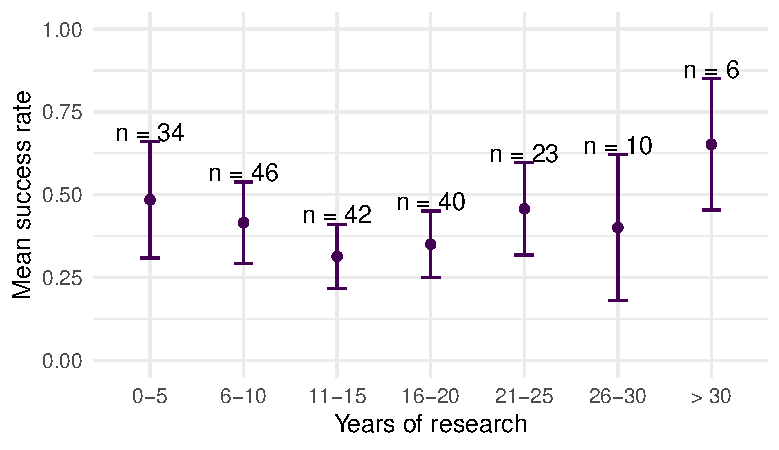
\includegraphics[keepaspectratio]{index_files/figure-pdf/fig-success-1.pdf}}

}

\caption{\label{fig-success}\textbf{Distribution of participants'
success rate by year of research experience.} Above error bars n
represents the number of participants.}

\end{figure}%

\textsubscript{Source:
\href{https://RLadies-BA.github.io/quarto-manuscripts/index-preview.html}{Article
Notebook}}

\textsubscript{Source:
\href{https://RLadies-BA.github.io/quarto-manuscripts/index-preview.html}{Article
Notebook}}

When asked about their usual practices in preparing grant applications,
the most commonly reported actions (rated ``always'') included reviewing
eligibility and call requirements (n = 151, 82.97\%), conducting a
detailed reading of the call guidelines and annexes (n = 143, 78.57\%),
and alignment of the project objectives with the call (n = 129,
70.88\%). Less frequently applied were practices such as requesting
feedback from colleagues (n = 84, 46.15\%), studying the profiles of
funder institutions and reviewers (n = 52, 28.57\%), and establishing
strategic partnerships with other institutions or researchers (n = 50,
27.47\%) (Fig~\ref{fig-practices}).

\protect\phantomsection\label{cell-fig-practices}
\begin{figure}[H]

\centering{

\pandocbounded{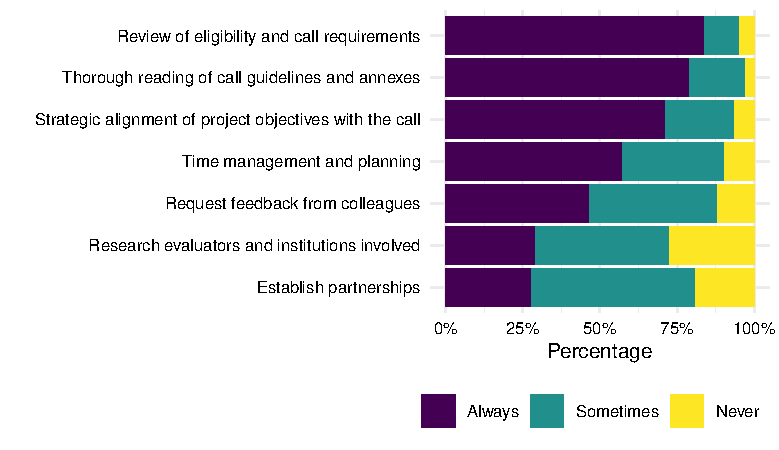
\includegraphics[keepaspectratio]{index_files/figure-pdf/fig-practices-1.pdf}}

}

\caption{\label{fig-practices}\textbf{Reported practices in preparing
grant applications.}}

\end{figure}%

\textsubscript{Source:
\href{https://RLadies-BA.github.io/quarto-manuscripts/index-preview.html}{Article
Notebook}}

\subsection{Perceived barriers to accessing international
funding}\label{perceived-barriers-to-accessing-international-funding}

\textsubscript{Source:
\href{https://RLadies-BA.github.io/quarto-manuscripts/index-preview.html}{Article
Notebook}}

Perceived barriers to international funding were assessed using a set of
10 Likert-scale items (n = 182 complete responses). The vast majority of
respondents identified economic barriers to attending international
networking events as a major obstacle to accessing international
research funding, with more than nine out of ten participants (n = 168,
92.31\%) agreeing or strongly agreeing with this statement. The
misalignment between the eligibility requirements of international calls
and local academic trajectories (e.g., time since Ph.D., position
titles) was endorsed by 80.77\% (n = 147) of respondents, and rhetorical
differences in writing style by 75.27\% (n = 137). Psychosocial and
perception-related barriers were also salient. Many reported perceiving
self-doubt in Latin American researchers regarding their capacity to
compete at an international level (n = 126, 69.23\%) and, at the same
time, not being accustomed to self-promotion practices (n = 124,
68.13\%). In addition, 60.44\% (n = 110) highlighted biased perceptions
from funders about Latin American scientific and infrastructural
capabilities as a barrier. Language-related challenges were endorsed by
just over half of participants, with 53.85\% (n = 98) reporting the use
of a non-native language as a barrier (Fig~\ref{fig-barriers}).

\protect\phantomsection\label{cell-fig-barriers}
\begin{figure}[H]

\centering{

\pandocbounded{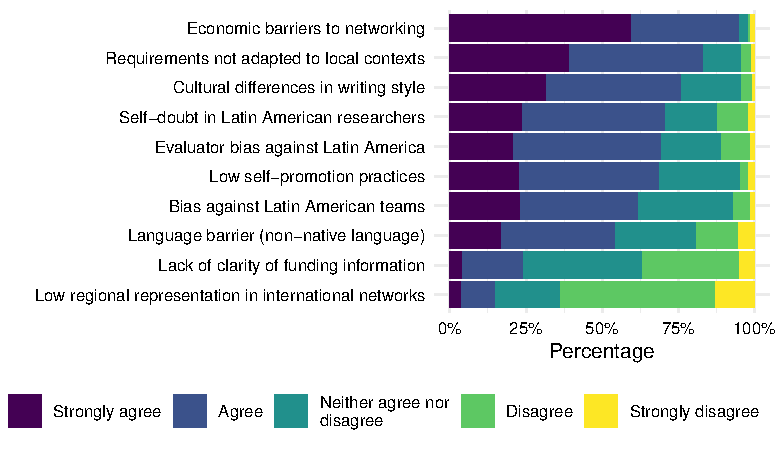
\includegraphics[keepaspectratio]{index_files/figure-pdf/fig-barriers-1.pdf}}

}

\caption{\label{fig-barriers}\textbf{Perceived barriers to accessing
international research funding among Latin American researchers.}}

\end{figure}%

\textsubscript{Source:
\href{https://RLadies-BA.github.io/quarto-manuscripts/index-preview.html}{Article
Notebook}}

By contrast, few participants identified issues of clarity in funding
information (n = 42, 23.08\%) or low regional representation in
international networks (n = 26, 14.29\%) as critical barriers.

Open-ended responses (n = 47, 25.82\%) highlighted additional barriers.
Specifically, the misalignment between Global North funders' agendas and
local priorities; limited training on how funders operate and make
decisions; structural exclusion through elitist or closed research
networks; bureaucratic hurdles due to lack of institutional support and
difficulties receiving international transfers. Respondents also noted
visibility constraints due to limited access to open-access publishing
and bibliographic databases, as well as limited familiarity with
international evaluation metrics.

\section{Discussion}\label{discussion}

Over the past decades, Latin America has made notable advances in
scientific productivity, with an increasing number of publications and
strengthened research networks. Nevertheless, researchers in the region
continue to operate under structural conditions that shape their
competitiveness in international funding environments in ways that
differ from those of researchers based in HICs {[}12{]}. Linguistic,
institutional, and contextual factors intersect to influence how Latin
American researchers prepare, submit, and experience international grant
applications {[}28{]}.

In this study, we use a mixed-methods design to examine barriers to
international research funding among Latin American researchers. The
focus group qualitative analysis, together with survey responses to
closed and open-ended questions, converged on similar structural and
procedural challenges. Consistent with previous research
{[}17,29--31{]}, the requirement to write grant proposals in English
emerged as a key barrier. Participants described how this linguistic
demand not only compromises the clarity and persuasiveness of proposals
but also reinforces perceptions of lower competitiveness. Cultural
differences in rhetorical conventions further influence proposal
development, as international funders often prioritize concise,
action-oriented writing styles that may differ from the more expository
or theory-driven traditions prevalent in the region {[}30,31{]}.

Participants also highlighted how features of grant review processes can
interact with these linguistic and cultural dynamics. Evaluation
criteria and review norms developed within predominantly
English-speaking contexts may inadvertently disadvantage researchers
from historically underrepresented regions and groups {[}29,32{]}. This,
together with psychosocial factors such as self-doubt and regional norms
that sanction overt self-promotion, was described as shaping proposals
where applicants hedge claims, default to passive voice and collective
authorship, understate outcomes and novelty, avoid explicit asks
regarding budget and resources, and omit quantifiable milestones and
track record highlights. Reviewers may read these features as lower
confidence, feasibility, and leadership.

These findings underscore that grant writing differs significantly from
academic writing and constitutes a specialized professional skill that
requires specific training and institutional support {[}33{]}. However,
the lack of accessible training programs in Spanish or Portuguese that
address both linguistic and cultural mismatches further limits Latin
American researchers' ability to compete on equal footing with their
peers in the Global North. Training or offering support in writing and
framing proposals, tailored to international rhetorical expectations
while maintaining local voices and their relevance, may help mitigate
the disadvantages associated with cultural style differences.

Our analyses also underscored visibility and dissemination constraints
that respondents perceived as directly limiting their chances of
securing funding. In line with Boudry {[}34{]}, respondents pointed to
paywalled literature and to open-access processing charges (APCs) as
structural barriers that disproportionately impact LMIC authors, as they
skew who gets read and cited. Respondents also linked limited visibility
to difficulties attending networking events, which, in turn, diminishes
their access to opportunities. This coincides with Mocanu et al.
{[}35{]}, which concludes that what predicts the success of grant
applications is, largely, the PI's previous publications and their
international visibility. Enabling travel grants, virtual partnering,
and mentorship linking applicants with experienced PIs could mitigate
these limitations.

Administrative load and weak institutional support also emerged as
another limiting factor. As suggested by previous studies {[}36--38{]},
substantial administrative burden in grant preparation and management
diverts time from research, and this disproportionately impacts
less-resourced institutions {[}39{]}. Including LMIC experts in the
design of funding calls, calibrating expectations about organisational
models, and valuing contextual knowledge may reduce the current
asymmetries {[}40{]}.

Beyond linguistic and cultural factors, several structural features of
the global research funding landscape continue to shape Latin American
researchers' participation in international funding competitions
{[}40{]}. While international funding schemes are not designed to
address structural disparities between research systems, some funding
organizations have begun to explore ways of promoting diversity and
broader participation within the global research ecosystem. Current and
former initiatives by funders such as the Wellcome Trust, the
International Development Research Centre (IDRC), the Gates Foundation,
and the Chan Zuckerberg Initiative illustrate an emerging interest in
equity, diversity, and inclusion (EDI). Although a systematic assessment
of such initiatives falls outside the scope of this study, our findings
highlight the importance of evidence-informed approaches to
understanding how structural conditions shape researchers' experiences.
In this context, the development of standardized indicators and
transparent data collection practices may help assess the effects of
EDI-oriented measures and clarify how different support mechanisms
interact with existing funding processes, particularly for researchers
based in LMICs {[}41{]}.

This work has some limitations that should be taken into consideration
when interpreting the results. First, the measures rely on self-report;
we did not independently verify the number of submissions or awards, nor
did we track proposals and career paths longitudinally. As a result,
recall bias and social desirability bias cannot be ruled out. Second,
the analysis focuses primarily on funding success and perceived barriers
in international grant competitions. We did not examine other relevant
indicators of research outcomes, such as reviewer scores, subsequent
network development, or publication trajectories, which may capture
additional benefits associated with applying for international funding.
Third, our sample over-represents researchers based in Argentina,
reducing regional generalizability. Finally, several challenges
discussed in this study---such as limited research infrastructure,
institutional capacity constraints, and administrative burdens---are
closely linked to domestic science policy contexts. These factors fall
in part outside the scope of international funding design and cannot be
readily addressed through modifications to international funding schemes
alone.

Taken together, the present findings contribute to a more nuanced
understanding of how structural conditions shape researchers'
competitiveness in international funding environments and where
targeted, feasible forms of support may be most effective. Enabling
mechanisms informed by the experiences of Latin American researchers,
such as those focused on proposal preparation, institutional capacity,
and navigation of funding processes, have the potential to strengthen
researchers' preparedness for international funding competitions in the
near to mid term. Future work should build on these findings and assess
the impact of potential interventions.

\protect\phantomsection\label{refs}
\begin{CSLReferences}{0}{1}
\bibitem[\citeproctext]{ref-ref01}
\CSLLeftMargin{1. }%
\CSLRightInline{Rivera-Lozada O, Yangali-Vicente JS, Millones-Gòmez PA,
Minchón-Medina CA, Rosales-Cifuentes TV. Impact of economic growth on
scientific production in {Latin America} and the {Caribbean} based on
panel data analysis. F1000Res. 2023;12: 242.
doi:\href{https://doi.org/10.12688/f1000research.128075.1}{10.12688/f1000research.128075.1}}

\bibitem[\citeproctext]{ref-ref02}
\CSLLeftMargin{2. }%
\CSLRightInline{Chinchilla-Rodríguez Z, Miao L, Murray D,
Robinson-García N, Costas R, Sugimoto CR. A global comparison of
scientific mobility and collaboration according to national scientific
capacities. Front Res Metr Anal. 2018;3.
doi:\href{https://doi.org/10.3389/frma.2018.00017}{10.3389/frma.2018.00017}}

\bibitem[\citeproctext]{ref-ref03}
\CSLLeftMargin{3. }%
\CSLRightInline{Murray M, Mubiligi J. An approach to building equitable
global health research collaborations. Ann Glob Health. 2020;86: 126.
doi:\href{https://doi.org/10.5334/aogh.3039}{10.5334/aogh.3039}}

\bibitem[\citeproctext]{ref-ref04}
\CSLLeftMargin{4. }%
\CSLRightInline{Edwards MA, Roy S. Academic research in the 21st
century: Maintaining scientific integrity in a climate of perverse
incentives and hypercompetition. Environ Eng Sci. 2017;34: 51--61.
doi:\href{https://doi.org/10.1089/ees.2016.0223}{10.1089/ees.2016.0223}}

\bibitem[\citeproctext]{ref-ref05}
\CSLLeftMargin{5. }%
\CSLRightInline{Skupien S, Rüffin N. The geography of research funding:
Semantics and beyond. J Stud Int Educ. 2019;24: 24--38.
doi:\href{https://doi.org/10.1177/1028315319889896}{10.1177/1028315319889896}}

\bibitem[\citeproctext]{ref-ref06}
\CSLLeftMargin{6. }%
\CSLRightInline{World Bank. Research and development expenditure (\% of
{GDP}) {[}internet{]}. Available: \url{https://data.worldbank.org}}

\bibitem[\citeproctext]{ref-ref07}
\CSLLeftMargin{7. }%
\CSLRightInline{Santa S, Herrero Solana V. Producci{ó}n cient{í}fica de
{Am{é}rica Latina} y el {Caribe}: Una aproximaci{ó}n a trav{é}s de los
datos de {Scopus} (1996--2007). Rev Interam Bibliotecol. 2010;33:
379--400. }

\bibitem[\citeproctext]{ref-ref08}
\CSLLeftMargin{8. }%
\CSLRightInline{Sterling-Sandor L. Exploring correlations between
governmental expenditure in research and development and productivity in
{Latin America} {[}internet{]}. 2025. Available:
\url{https://urn.kb.se/resolve?urn=urn:nbn:se:umu:diva-240138}}

\bibitem[\citeproctext]{ref-ref09}
\CSLLeftMargin{9. }%
\CSLRightInline{Morciano C, Errico MC, Faralli C, Minghetti L. An
analysis of the strategic plan development processes of major public
organisations funding health research in nine high-income countries
worldwide. Health Res Policy Syst. 2020;18: 106.
doi:\href{https://doi.org/10.1186/s12961-020-00620-x}{10.1186/s12961-020-00620-x}}

\bibitem[\citeproctext]{ref-ref10}
\CSLLeftMargin{10. }%
\CSLRightInline{Tanyu NR. International research funding in {African}
higher education: Risks and benefits. Int High Educ. 2025;122: 9--10. }

\bibitem[\citeproctext]{ref-ref11}
\CSLLeftMargin{11. }%
\CSLRightInline{Head MG, Brown RJ, Newell ML, Scott JAG, Batchelor J,
Atun R. The allocation of {US}\$105 billion in global funding from {G20}
countries for infectious disease research between 2000 and 2017: A
content analysis of investments. Lancet Glob Health. 2020;8:
e1295--e1304.
doi:\href{https://doi.org/10.1016/S2214-109X(20)30312-0}{10.1016/S2214-109X(20)30312-0}}

\bibitem[\citeproctext]{ref-ref12}
\CSLLeftMargin{12. }%
\CSLRightInline{Charani E, Abimbola S, Pai M, Adeyi O, Mendelson M,
Laxminarayan R. Funders: The missing link in equitable global health
research? PLOS Glob Public Health. 2022;2: e0000583.
doi:\href{https://doi.org/10.1371/journal.pgph.0000583}{10.1371/journal.pgph.0000583}}

\bibitem[\citeproctext]{ref-ref13}
\CSLLeftMargin{13. }%
\CSLRightInline{Di Bitetti MS, Ferreras JA. Publish (in {English}) or
perish: The effect on citation rate of using languages other than
{English} in scientific publications. Ambio. 2017;46: 121--127.
doi:\href{https://doi.org/10.1007/s13280-016-0820-7}{10.1007/s13280-016-0820-7}}

\bibitem[\citeproctext]{ref-ref14}
\CSLLeftMargin{14. }%
\CSLRightInline{Liu W. The changing role of non-{English} papers in
scholarly communication: Evidence from {Web of Science}'s three journal
citation indexes. Learn Publ. 2016;30: 115--123.
doi:\href{https://doi.org/10.1002/leap.1089}{10.1002/leap.1089}}

\bibitem[\citeproctext]{ref-ref15}
\CSLLeftMargin{15. }%
\CSLRightInline{Gomez CJ, Herman AC, Parigi P. Leading countries in
global science increasingly receive more citations than other countries
doing similar research. Nat Hum Behav. 2022;6: 919--929.
doi:\href{https://doi.org/10.1038/s41562-022-01351-5}{10.1038/s41562-022-01351-5}}

\bibitem[\citeproctext]{ref-ref16}
\CSLLeftMargin{16. }%
\CSLRightInline{Verma P. The role of {English} in academic writing:
Strategies for non-native speakers. J Int Engl Res Stud. 2023;1: 35--40.
}

\bibitem[\citeproctext]{ref-ref17}
\CSLLeftMargin{17. }%
\CSLRightInline{Pascual M, Unger L. Appraisal in the research genres: An
analysis of grant proposals by {Argentinean} researchers. Rev signos.
2010;43.
doi:\href{https://doi.org/10.4067/s0718-09342010000200004}{10.4067/s0718-09342010000200004}}

\bibitem[\citeproctext]{ref-ref18}
\CSLLeftMargin{18. }%
\CSLRightInline{Hanauer DI, Sheridan CL, Englander K. Linguistic
injustice in the writing of research articles in {English} as a second
language: Data from {Taiwanese} and {Mexican} researchers. Writ Commun.
2019;36: 136--154. }

\bibitem[\citeproctext]{ref-ref19}
\CSLLeftMargin{19. }%
\CSLRightInline{De Winde CM, Sarabipour S, Carignano H, Davla S, Eccles
D, Hainer SJ. Towards inclusive funding practices for early career
researchers. J Sci Policy Gov {[}Internet{]}. 2021;18(01); Available:
\url{https://www.sciencepolicyjournal.org/article_1038126_jspg180105}}

\bibitem[\citeproctext]{ref-ref20}
\CSLLeftMargin{20. }%
\CSLRightInline{Valenzuela-Toro AM, Viglino M. How {Latin American}
researchers suffer in science. Nature. 2021;598: 374--375.
doi:\href{https://doi.org/10.1038/d41586-021-02601-8}{10.1038/d41586-021-02601-8}}

\bibitem[\citeproctext]{ref-ref21}
\CSLLeftMargin{21. }%
\CSLRightInline{{Jones HP, McGee R, Weber-Main AM, Buchwald DS, Manson
SM, Vishwanatha JK, et al.} Enhancing research careers: An example of a
{US} national diversity-focused, grant-writing training and coaching
experiment. BMC Proc. 2017;11: 16.
doi:\href{https://doi.org/10.1186/s12919-017-0084-7}{10.1186/s12919-017-0084-7}}

\bibitem[\citeproctext]{ref-ref22}
\CSLLeftMargin{22. }%
\CSLRightInline{Zacca-González G, Chinchilla-Rodríguez Z, Vargas-Quesada
B, Moya-Anegón F de. Bibliometric analysis of regional {Latin America}'s
scientific output in {Public Health} through {SCImago Journal \& Country
Rank}. BMC Public Health. 2014;14: 632.
doi:\href{https://doi.org/10.1186/1471-2458-14-632}{10.1186/1471-2458-14-632}}

\bibitem[\citeproctext]{ref-ref23}
\CSLLeftMargin{23. }%
\CSLRightInline{Huete-Perez JA, Salvatierra N. Assessing biomedical
research capacities in selected countries of {Latin America}:
Challenges, opportunities, and recommendations. Front Res Metr Anal.
2025;10: 1594303.
doi:\href{https://doi.org/10.3389/frma.2025.1594303}{10.3389/frma.2025.1594303}}

\bibitem[\citeproctext]{ref-ref24}
\CSLLeftMargin{24. }%
\CSLRightInline{Braun V, Clarke V. Using thematic analysis in
psychology. Qual Res Psychol. 2006;3: 77--101. }

\bibitem[\citeproctext]{ref-ref25}
\CSLLeftMargin{25. }%
\CSLRightInline{Boyatzis R. Transforming qualitative information:
Thematic analysis and code development. Sage; 1998. }

\bibitem[\citeproctext]{ref-ref26}
\CSLLeftMargin{26. }%
\CSLRightInline{Taylor GW, Ussher JM. Making sense of {S\&M}: A
discourse analytic account. Sexualities. 2001;4: 293--314. }

\bibitem[\citeproctext]{ref-ref27}
\CSLLeftMargin{27. }%
\CSLRightInline{R Core Team. R: A language and environment for
statistical computing {[}internet{]}. Vienna, Austria: R Foundation for
Statistical Computing; 2024; Available:
\url{https://www.r-project.org/}}

\bibitem[\citeproctext]{ref-ref28}
\CSLLeftMargin{28. }%
\CSLRightInline{Estenssoro E, Friedman G, Hernández G. Research in
{Latin America}: Opportunities and challenges. Intensive Care Med.
2016;42: 1045--1047.
doi:\href{https://doi.org/10.1007/s00134-016-4342-3}{10.1007/s00134-016-4342-3}}

\bibitem[\citeproctext]{ref-ref29}
\CSLLeftMargin{29. }%
\CSLRightInline{Ruediger S, Ris L, Iyer K. Equitable research funding:
Strategies, challenges and the role of funding agencies. Eur J Neurosci.
2025;61: e70160.
doi:\href{https://doi.org/10.1111/ejn.70160}{10.1111/ejn.70160}}

\bibitem[\citeproctext]{ref-ref30}
\CSLLeftMargin{30. }%
\CSLRightInline{Besselaar P van den, Mom C. The effect of writing style
on success in grant applications. J Informetr. 2022;16: 101257. }

\bibitem[\citeproctext]{ref-ref31}
\CSLLeftMargin{31. }%
\CSLRightInline{Boyack KW, Smith C, Klavans R. Toward predicting
research proposal success. Scientometrics. 2018;114: 449--461. }

\bibitem[\citeproctext]{ref-ref32}
\CSLLeftMargin{32. }%
\CSLRightInline{Stoop C, Belou R, Smith JL. Facilitating the success of
women's early career grants: A local solution to a national problem.
Innov High Educ. 2023;48: 907--924. }

\bibitem[\citeproctext]{ref-ref33}
\CSLLeftMargin{33. }%
\CSLRightInline{Glowacki S, Nims J, Liggit P. Determining the impact of
grant writing workshops on faculty learning. IJournal Res Adm
{[}Internet{]}. 2020; Available:
\url{https://commons.emich.edu/fac_sch2020/335}}

\bibitem[\citeproctext]{ref-ref34}
\CSLLeftMargin{34. }%
\CSLRightInline{Boudry C, Alvarez-Muñoz P, Arencibia-Jorge R, Ayena D,
Brouwer NJ, Chaudhuri Z. Worldwide inequality in access to full text
scientific articles: The example of ophthalmology. PeerJ. 2019;7: e7850.
doi:\href{https://doi.org/10.7717/peerj.7850}{10.7717/peerj.7850}}

\bibitem[\citeproctext]{ref-ref35}
\CSLLeftMargin{35. }%
\CSLRightInline{Mocanu M, Rusu VD, Bibiri A-D. Competing for research
funding: Key elements impacting the evaluation of grant proposal.
Heliyon. 2024;10: e36015.
doi:\href{https://doi.org/10.1016/j.heliyon.2024.e36015}{10.1016/j.heliyon.2024.e36015}}

\bibitem[\citeproctext]{ref-ref36}
\CSLLeftMargin{36. }%
\CSLRightInline{Herbert DL, Barnett AG, Clarke P, Graves N. On the time
spent preparing grant proposals: An observational study of {Australian}
researchers. BMJ Open. 2013;3: e002800.
doi:\href{https://doi.org/10.1136/bmjopen-2013-002800}{10.1136/bmjopen-2013-002800}}

\bibitem[\citeproctext]{ref-ref37}
\CSLLeftMargin{37. }%
\CSLRightInline{Hippel T von, Hippel C von. To apply or not to apply: A
survey analysis of grant writing costs and benefits. PLoS One. 2015;10:
e0118494.
doi:\href{https://doi.org/10.1371/journal.pone.0118494}{10.1371/journal.pone.0118494}}

\bibitem[\citeproctext]{ref-ref38}
\CSLLeftMargin{38. }%
\CSLRightInline{Gross K, Bergstrom CT. Contest models highlight inherent
inefficiencies of scientific funding competitions. PLoS Biol. 2019;17:
e3000065.
doi:\href{https://doi.org/10.1371/journal.pbio.3000065}{10.1371/journal.pbio.3000065}}

\bibitem[\citeproctext]{ref-ref39}
\CSLLeftMargin{39. }%
\CSLRightInline{Rockwell S. The {FDP} faculty burden survey. Research
Manag Rev. 2009;16(2):29--44; Available:
\url{https://pmc.ncbi.nlm.nih.gov/articles/PMC2887040/pdf/nihms-156127.pdf}}

\bibitem[\citeproctext]{ref-ref40}
\CSLLeftMargin{40. }%
\CSLRightInline{Koum Besson ES. How to identify epistemic injustice in
global health research funding practices: A decolonial guide. BMJ Global
Health. 2022;7: e008950.
doi:\href{https://doi.org/10.1136/bmjgh-2021-008950}{10.1136/bmjgh-2021-008950}}

\bibitem[\citeproctext]{ref-ref41}
\CSLLeftMargin{41. }%
\CSLRightInline{Franco MC, Rice DB, Schuch HS, Dellagostin OA, Cenci MS,
Moher D. The impact of gender on scientific writing: An observational
study of grant proposals. J Clin Epidemiol. 2021;136: 37--43. }

\end{CSLReferences}




\end{document}
